\documentclass[12pt,a4paper]{article}

% Packages
\usepackage[utf8]{inputenc}
\usepackage[margin=0.5in,landscape]{geometry}
\usepackage{tikz}
\usetikzlibrary{shapes.geometric, arrows.meta, positioning, fit, calc, backgrounds, shapes.multipart, decorations.pathreplacing}
\usepackage{xcolor}
\usepackage{amsmath}

% Define colors
\definecolor{moduleblue}{RGB}{100,149,237}
\definecolor{modulegray}{RGB}{220,220,220}
\definecolor{signalred}{RGB}{220,20,60}
\definecolor{signalgreen}{RGB}{34,139,34}
\definecolor{statecolor}{RGB}{255,218,185}
\definecolor{keycolor}{RGB}{255,255,153}

% TikZ styles
\tikzstyle{module} = [rectangle, rounded corners, minimum width=3cm, minimum height=1cm, text centered, draw=black, fill=moduleblue!30, font=\small\ttfamily]
\tikzstyle{submodule} = [rectangle, rounded corners, minimum width=2.5cm, minimum height=0.8cm, text centered, draw=black, fill=modulegray, font=\scriptsize\ttfamily]
\tikzstyle{smallmodule} = [rectangle, rounded corners, minimum width=2cm, minimum height=0.6cm, text centered, draw=black, fill=modulegray, font=\tiny\ttfamily]
\tikzstyle{state} = [ellipse, minimum width=2cm, minimum height=1cm, text centered, draw=black, fill=statecolor, font=\scriptsize]
\tikzstyle{arrow} = [thick,->,>=Stealth]
\tikzstyle{dataarrow} = [thick,->,>=Stealth,color=signalred]
\tikzstyle{controlarrow} = [thick,->,>=Stealth,color=signalgreen]
\tikzstyle{bus} = [very thick,->,>=Stealth,color=blue]
\tikzstyle{input} = [trapezium, trapezium left angle=70, trapezium right angle=110, minimum width=2cm, minimum height=0.8cm, text centered, draw=black, fill=green!20, font=\small]
\tikzstyle{output} = [trapezium, trapezium left angle=110, trapezium right angle=70, minimum width=2cm, minimum height=0.8cm, text centered, draw=black, fill=red!20, font=\small]

\title{\textbf{AES-128 FPGA Implementation}\\Architecture Diagrams}
\author{}
\date{}

\begin{document}

\maketitle

%==============================================================================
% PAGE 1: Top-Level System Architecture
%==============================================================================
\begin{figure}[p]
\centering
\begin{tikzpicture}[node distance=2cm, scale=0.9, every node/.style={transform shape}]

% Title
\node[font=\Large\bfseries] at (0,9) {Top-Level System Architecture};

% FPGA Board peripherals (left side - inputs)
\node[input] (clk) at (-8,7) {clk (100MHz)};
\node[input] (rst) at (-8,5.5) {rst\_n};
\node[input] (btnC) at (-8,4) {btnC (start)};
\node[input] (btnU) at (-8,3) {btnU (enc/dec)};
\node[input] (btnLR) at (-8,2) {btnL/R (display)};
\node[input] (sw) at (-8,0.5) {sw[15:0] (test)};

% Main top module
\node[module, minimum width=14cm, minimum height=8cm] (top) at (0,3) {};
\node[font=\large\bfseries] at (0,6.8) {aes\_fpga\_top};

% Button control
\node[submodule, minimum width=4cm] (debounce) at (-3,5.5) {Button Debouncing\\Edge Detection};

% Test vector selection
\node[submodule, minimum width=4cm] (testvec) at (-3,3.5) {Test Vector\\Selection Logic};

% AES Core (main component)
\node[module, minimum width=5cm, minimum height=5cm, fill=moduleblue!50] (aes_core) at (2,3) {};
\node[font=\bfseries] at (2,5) {aes\_core\_fixed};

% Internal AES components
\node[smallmodule, minimum width=4cm] (fsm) at (2,4.3) {State Machine};
\node[smallmodule] (key_exp) at (2,3.5) {Key Expansion};
\node[smallmodule] (subbytes) at (2,2.7) {SubBytes};
\node[smallmodule] (shiftrows) at (2,1.9) {ShiftRows};
\node[smallmodule] (mixcols) at (2,1.1) {MixColumns};

% Seven segment controller
\node[submodule, minimum width=3cm] (seg_ctrl) at (-3,0.5) {Seven Segment\\Controller};

% FPGA Board peripherals (right side - outputs)
\node[output] (led) at (8,5) {led[15:0]};
\node[output] (an) at (8,2.5) {an[7:0]};
\node[output] (seg) at (8,1) {seg[6:0]};

% Arrows - inputs to modules
\draw[arrow] (clk) -- (-5,7) -- (-5,5.5) -- (debounce);
\draw[arrow] (rst) -- (debounce);
\draw[arrow] (btnC) -- (debounce);
\draw[arrow] (btnU) -- (debounce);
\draw[arrow] (btnLR) -- (debounce);
\draw[arrow] (sw) -- (testvec);

% Arrows - internal connections
\draw[arrow] (debounce) -- node[above,font=\tiny] {start, mode} (-1,5.5) -- (-1,4.5) -- (fsm);
\draw[arrow] (testvec) -- node[above,font=\tiny] {plaintext[127:0]} (-1,3.5) -- (1,3.5) -- (fsm);
\draw[arrow] (testvec) -- node[above,font=\tiny] {key[127:0]} (0.5,3.5);

% AES Core to display
\draw[bus] (aes_core) -- node[above,font=\tiny] {data\_out[127:0]} (-1,2.5) -- (-1,0.8) -- (seg_ctrl);
\draw[arrow] (debounce) -- (-4,5.5) -- (-4,1) -- (seg_ctrl);

% Outputs
\draw[arrow] (seg_ctrl) -- node[above,font=\tiny] {an[7:0]} (5,0.5) -- (5,2.5) -- (an);
\draw[arrow] (seg_ctrl) -- node[above,font=\tiny] {seg[6:0]} (6,0.5) -- (6,1) -- (seg);
\draw[arrow] (aes_core) -- node[above,font=\tiny] {ready, status} (5,3) -- (5,5) -- (led);
\draw[arrow] (debounce) -- (5.5,5.5) -- (5.5,5) -- (led);

% Legend
\node[draw, rectangle, fill=white, align=left, font=\scriptsize] at (0,-2) {
\textbf{Signal Types:}\\
\textcolor{black}{━━━} Control signals\\
\textcolor{blue}{\textbf{━━━}} Data buses (128-bit)\\
\textcolor{signalgreen}{\textbf{━━━}} Control flow\\
\textcolor{signalred}{\textbf{━━━}} Data flow
};

\end{tikzpicture}
\caption{Top-level FPGA system showing I/O interface and main modules}
\end{figure}

%==============================================================================
% PAGE 2: AES Core Internal Architecture
%==============================================================================
\begin{figure}[p]
\centering
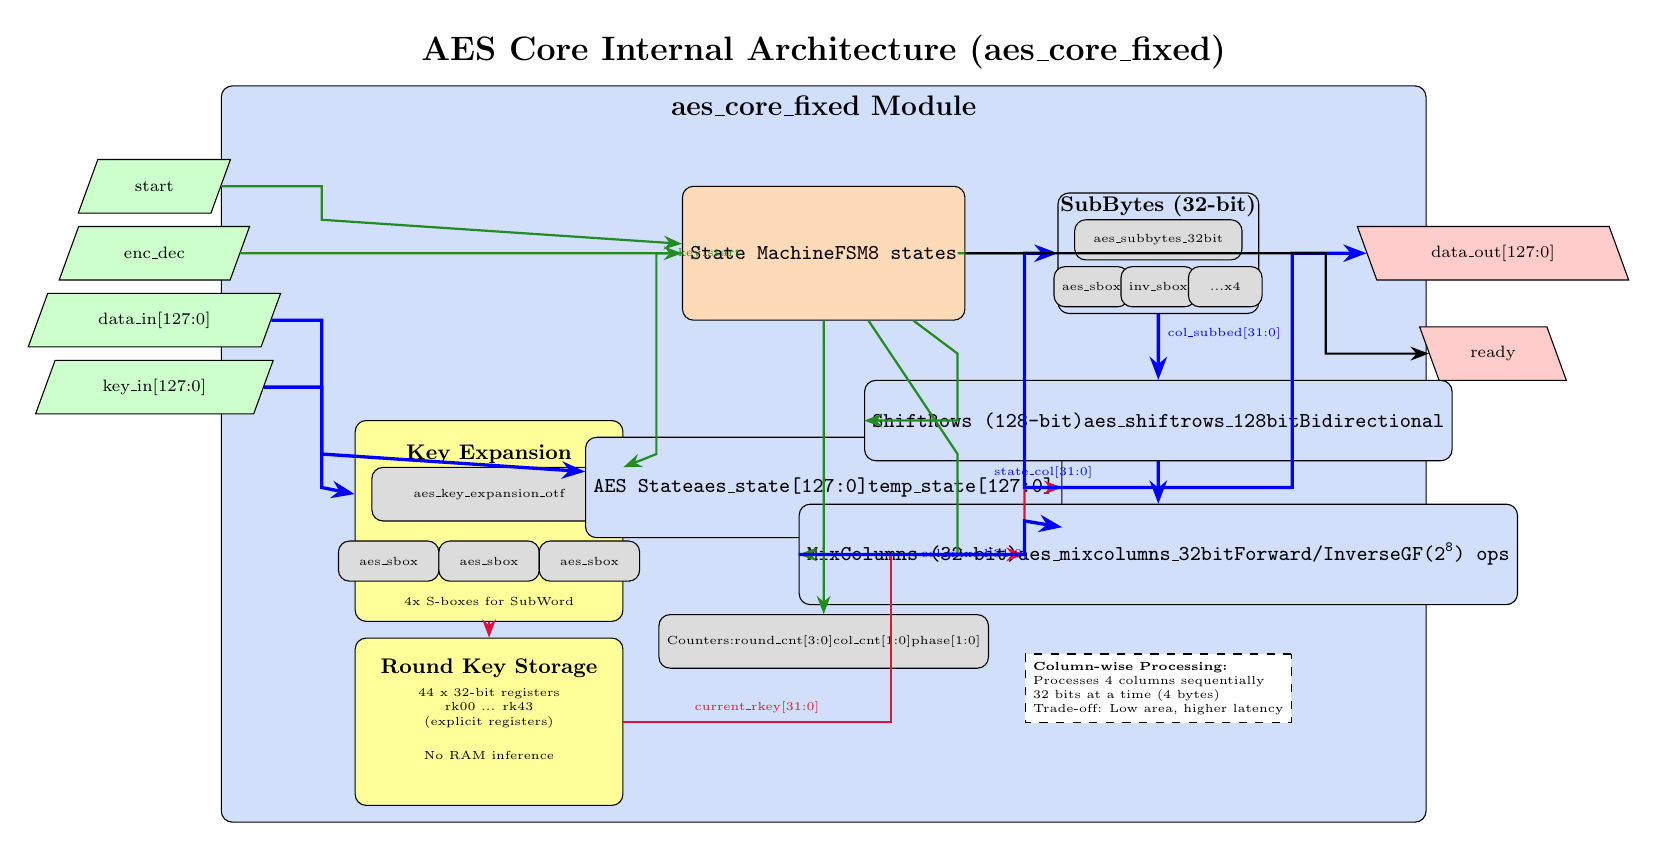
\begin{tikzpicture}[node distance=1.5cm, scale=0.85, every node/.style={transform shape}]

% Title
\node[font=\Large\bfseries] at (0,10) {AES Core Internal Architecture (aes\_core\_fixed)};

% Core boundary
\node[module, minimum width=18cm, minimum height=11cm] (core_boundary) at (0,4) {};
\node[font=\large\bfseries] at (0,9.2) {aes\_core\_fixed Module};

% Inputs
\node[input, font=\scriptsize] (start_in) at (-10,8) {start};
\node[input, font=\scriptsize] (enc_dec_in) at (-10,7) {enc\_dec};
\node[input, font=\scriptsize] (data_in) at (-10,6) {data\_in[127:0]};
\node[input, font=\scriptsize] (key_in) at (-10,5) {key\_in[127:0]};

% State Machine (central control)
\node[module, minimum width=3cm, minimum height=2cm, fill=statecolor] (fsm) at (0,7) {State Machine\\FSM\\8 states};

% Key Expansion Module
\node[module, minimum width=4cm, minimum height=3cm, fill=keycolor] (key_module) at (-5,3) {};
\node[font=\small\bfseries] at (-5,4) {Key Expansion};
\node[submodule, minimum width=3.5cm, font=\tiny] (key_otf) at (-5,3.4) {aes\_key\_expansion\_otf};
\node[smallmodule, minimum width=1.5cm, font=\tiny] (sbox0) at (-6.5,2.4) {aes\_sbox};
\node[smallmodule, minimum width=1.5cm, font=\tiny] (sbox1) at (-5,2.4) {aes\_sbox};
\node[smallmodule, minimum width=1.5cm, font=\tiny] (sbox2) at (-3.5,2.4) {aes\_sbox};
\node[font=\tiny] at (-5,1.8) {4x S-boxes for SubWord};

% Round Key Storage
\node[module, minimum width=4cm, minimum height=2.5cm, fill=keycolor] (rkey_store) at (-5,0) {};
\node[font=\small\bfseries] at (-5,0.8) {Round Key Storage};
\node[font=\tiny, align=center] at (-5,0.2) {44 x 32-bit registers\\rk00 ... rk43\\(explicit registers)};
\node[font=\tiny] at (-5,-0.5) {No RAM inference};

% State Registers
\node[module, minimum width=3.5cm, minimum height=1.5cm] (state_reg) at (0,3.5) {AES State\\aes\_state[127:0]\\temp\_state[127:0]};

% SubBytes Module
\node[module, minimum width=3cm, minimum height=1.8cm] (subbytes_mod) at (5,7) {};
\node[font=\small\bfseries] at (5,7.7) {SubBytes (32-bit)};
\node[smallmodule, minimum width=2.5cm, font=\tiny] (sub_wrapper) at (5,7.2) {aes\_subbytes\_32bit};
\node[smallmodule, minimum width=1.1cm, font=\tiny] (sbox_fwd) at (4,6.5) {aes\_sbox};
\node[smallmodule, minimum width=1.1cm, font=\tiny] (sbox_inv) at (5,6.5) {inv\_sbox};
\node[smallmodule, minimum width=1.1cm, font=\tiny] (sbox_3) at (6,6.5) {...x4};

% ShiftRows Module
\node[module, minimum width=3cm, minimum height=1.2cm] (shiftrows_mod) at (5,4.5) {ShiftRows (128-bit)\\aes\_shiftrows\_128bit\\Bidirectional};

% MixColumns Module
\node[module, minimum width=3cm, minimum height=1.5cm] (mixcols_mod) at (5,2.5) {MixColumns (32-bit)\\aes\_mixcolumns\_32bit\\Forward/Inverse\\GF(2\textsuperscript{8}) ops};

% Counters and Control
\node[submodule, minimum width=2.5cm, font=\tiny] (counters) at (0,1.2) {Counters:\\round\_cnt[3:0]\\col\_cnt[1:0]\\phase[1:0]};

% Outputs
\node[output, font=\scriptsize] (data_out) at (10,7) {data\_out[127:0]};
\node[output, font=\scriptsize] (ready_out) at (10,5.5) {ready};

% Control signals
\draw[controlarrow] (start_in) -- (-7.5,8) -- (-7.5,7.5) -- (fsm);
\draw[controlarrow] (enc_dec_in) -- (-7,7) -- (fsm);

% Data inputs
\draw[bus] (data_in) -- (-7.5,6) -- (-7.5,4) -- (state_reg);
\draw[bus] (key_in) -- (-7.5,5) -- (-7.5,3.5) -- (key_module);

% FSM control to all modules
\draw[controlarrow] (fsm) -- node[right,font=\tiny] {key\_start} (-2.5,7) -- (-2.5,4) -- (key_module);
\draw[controlarrow] (fsm) -- (0,5.5) -- (counters);
\draw[controlarrow] (fsm) -- (2,7) -- (subbytes_mod);
\draw[controlarrow] (fsm) -- (2,5.5) -- (2,4.5) -- (shiftrows_mod);
\draw[controlarrow] (fsm) -- (2,4) -- (2,2.5) -- (mixcols_mod);

% Key expansion to storage
\draw[dataarrow] (key_module) -- (rkey_store);

% Round key to operations
\draw[dataarrow] (rkey_store) -- node[above,font=\tiny] {current\_rkey[31:0]} (1,0) -- (1,2.5) -- (3,2.5);
\draw[dataarrow] (3,2.5) -- (3,3.5) -- (state_reg);

% Data flow through operations
\draw[bus] (state_reg) -- node[above,font=\tiny] {state\_col[31:0]} (3,3.5) -- (3,7) -- (subbytes_mod);
\draw[bus] (subbytes_mod) -- node[right,font=\tiny] {col\_subbed[31:0]} (5,5.5) -- (shiftrows_mod);
\draw[bus] (shiftrows_mod) -- (shiftrows_mod |- mixcols_mod.north);
\draw[bus] (mixcols_mod) -- node[right,font=\tiny] {col\_mixed[31:0]} (3,2.5) -- (3,3) -- (state_reg);

% Output
\draw[bus] (state_reg) -- (7,3.5) -- (7,7) -- (data_out);
\draw[arrow] (fsm) -- (7.5,7) -- (7.5,5.5) -- (ready_out);

% Column processing annotation
\node[draw, rectangle, dashed, fill=white, align=left, font=\tiny] at (5,0.5) {
\textbf{Column-wise Processing:}\\
Processes 4 columns sequentially\\
32 bits at a time (4 bytes)\\
Trade-off: Low area, higher latency
};

\end{tikzpicture}
\caption{Detailed AES core architecture showing all internal modules and data paths}
\end{figure}

%==============================================================================
% PAGE 3: State Machine Diagram
%==============================================================================
\begin{figure}[p]
\centering
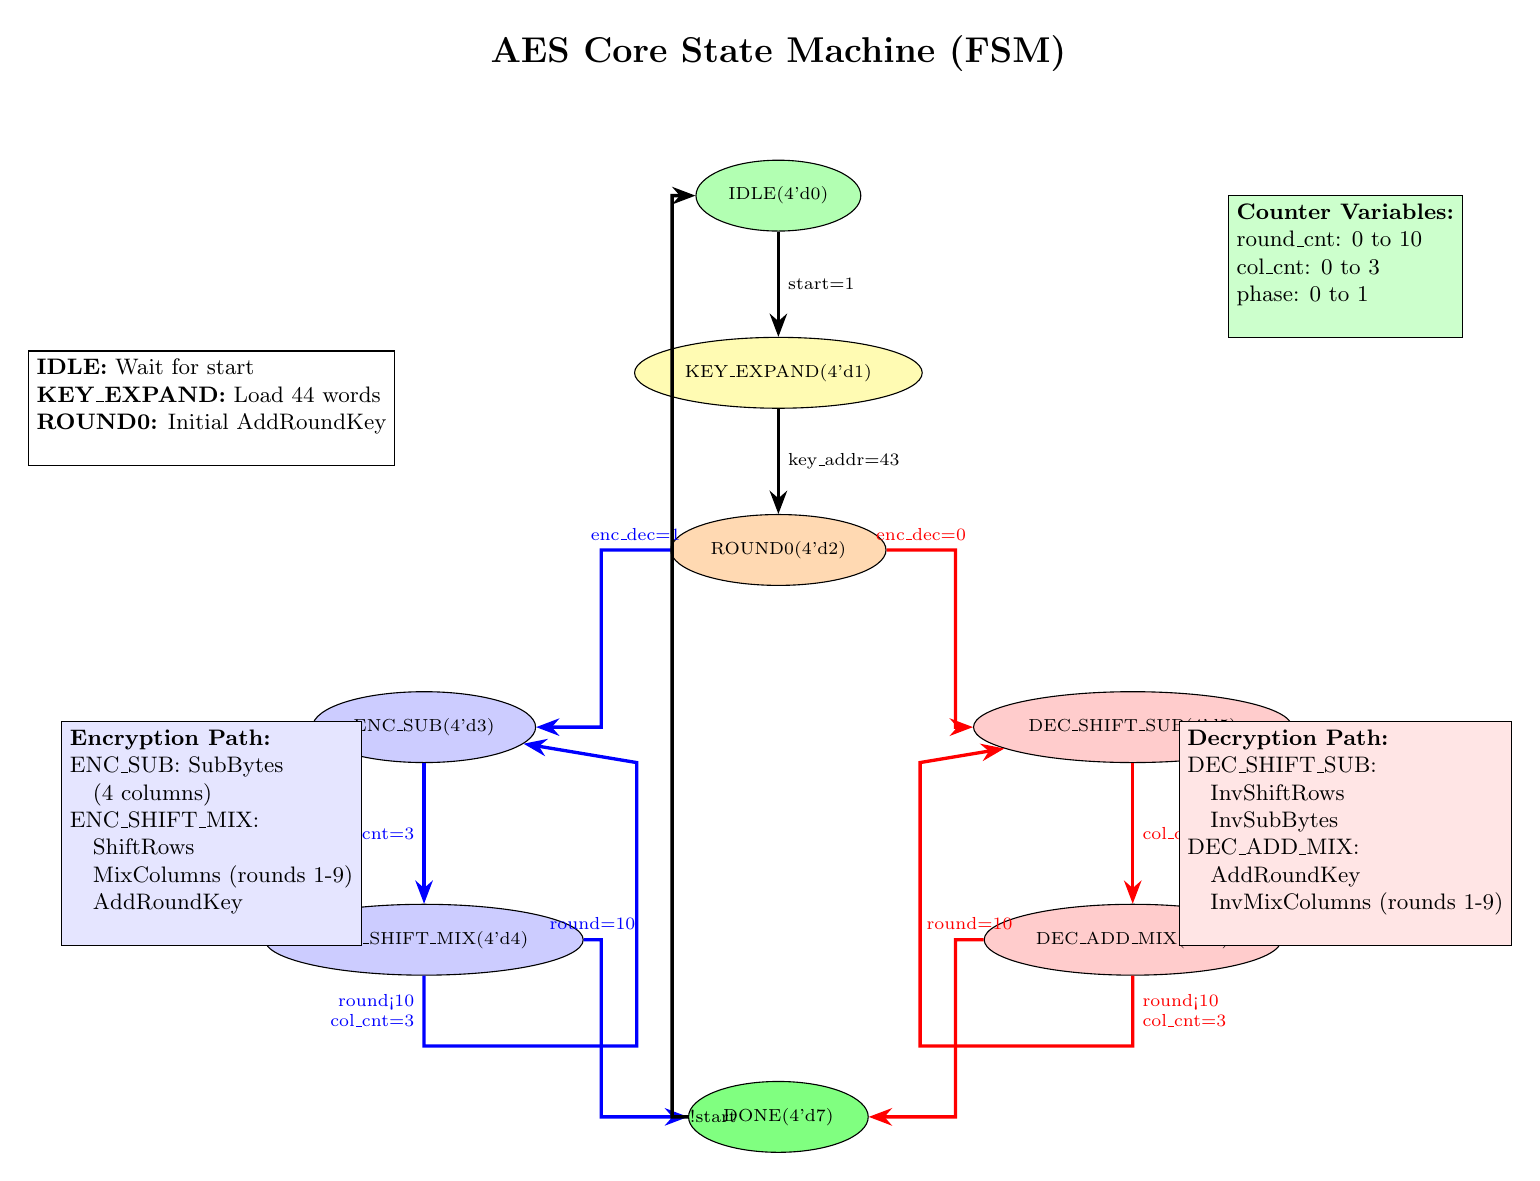
\begin{tikzpicture}[node distance=2.5cm, scale=0.9, every node/.style={transform shape}]

% Title
\node[font=\Large\bfseries] at (0,10) {AES Core State Machine (FSM)};

% States
\node[state, fill=green!30] (idle) at (0,8) {IDLE\\(4'd0)};
\node[state, fill=yellow!30] (keyexp) at (0,5.5) {KEY\_EXPAND\\(4'd1)};
\node[state, fill=orange!30] (round0) at (0,3) {ROUND0\\(4'd2)};

% Encryption path
\node[state, fill=blue!20] (enc_sub) at (-5,0.5) {ENC\_SUB\\(4'd3)};
\node[state, fill=blue!20] (enc_shift) at (-5,-2.5) {ENC\_SHIFT\_MIX\\(4'd4)};

% Decryption path
\node[state, fill=red!20] (dec_shift) at (5,0.5) {DEC\_SHIFT\_SUB\\(4'd5)};
\node[state, fill=red!20] (dec_add) at (5,-2.5) {DEC\_ADD\_MIX\\(4'd6)};

% Done state
\node[state, fill=green!50] (done) at (0,-5) {DONE\\(4'd7)};

% Transitions
\draw[arrow, very thick] (idle) -- node[right,font=\scriptsize] {start=1} (keyexp);
\draw[arrow, very thick] (keyexp) -- node[right,font=\scriptsize] {key\_addr=43} (round0);

% Encryption path
\draw[arrow, very thick, blue] (round0) -- node[above,font=\scriptsize] {enc\_dec=1} (-2.5,3) -- (-2.5,0.5) -- (enc_sub);
\draw[arrow, very thick, blue] (enc_sub) -- node[left,font=\scriptsize] {col\_cnt=3} (enc_shift);
\draw[arrow, very thick, blue] (enc_shift) -- node[left,font=\scriptsize,align=right] {round<10\\col\_cnt=3} (-5,-4) -- (-2,-4) -- (-2,0) -- (enc_sub);
\draw[arrow, very thick, blue] (enc_shift) -- node[above,font=\scriptsize] {round=10} (-2.5,-2.5) -- (-2.5,-5) -- (done);

% Decryption path
\draw[arrow, very thick, red] (round0) -- node[above,font=\scriptsize] {enc\_dec=0} (2.5,3) -- (2.5,0.5) -- (dec_shift);
\draw[arrow, very thick, red] (dec_shift) -- node[right,font=\scriptsize] {col\_cnt=3} (dec_add);
\draw[arrow, very thick, red] (dec_add) -- node[right,font=\scriptsize,align=left] {round<10\\col\_cnt=3} (5,-4) -- (2,-4) -- (2,0) -- (dec_shift);
\draw[arrow, very thick, red] (dec_add) -- node[above,font=\scriptsize] {round=10} (2.5,-2.5) -- (2.5,-5) -- (done);

% Return to IDLE
\draw[arrow, very thick] (done) -- node[right,font=\scriptsize] {!start} (-1.5,-5) -- (-1.5,8) -- (idle);

% Annotations
\node[draw, rectangle, fill=white, align=left, font=\small] at (-8,5) {
\textbf{IDLE:} Wait for start\\
\textbf{KEY\_EXPAND:} Load 44 words\\
\textbf{ROUND0:} Initial AddRoundKey\\
};

\node[draw, rectangle, fill=blue!10, align=left, font=\small] at (-8,-1) {
\textbf{Encryption Path:}\\
ENC\_SUB: SubBytes\\
\quad (4 columns)\\
ENC\_SHIFT\_MIX:\\
\quad ShiftRows\\
\quad MixColumns (rounds 1-9)\\
\quad AddRoundKey\\
};

\node[draw, rectangle, fill=red!10, align=left, font=\small] at (8,-1) {
\textbf{Decryption Path:}\\
DEC\_SHIFT\_SUB:\\
\quad InvShiftRows\\
\quad InvSubBytes\\
DEC\_ADD\_MIX:\\
\quad AddRoundKey\\
\quad InvMixColumns (rounds 1-9)\\
};

\node[draw, rectangle, fill=green!20, align=left, font=\small] at (8,7) {
\textbf{Counter Variables:}\\
round\_cnt: 0 to 10\\
col\_cnt: 0 to 3\\
phase: 0 to 1\\
};

\end{tikzpicture}
\caption{Complete state machine showing encryption and decryption paths}
\end{figure}

%==============================================================================
% PAGE 4: Key Expansion Architecture
%==============================================================================
\begin{figure}[p]
\centering
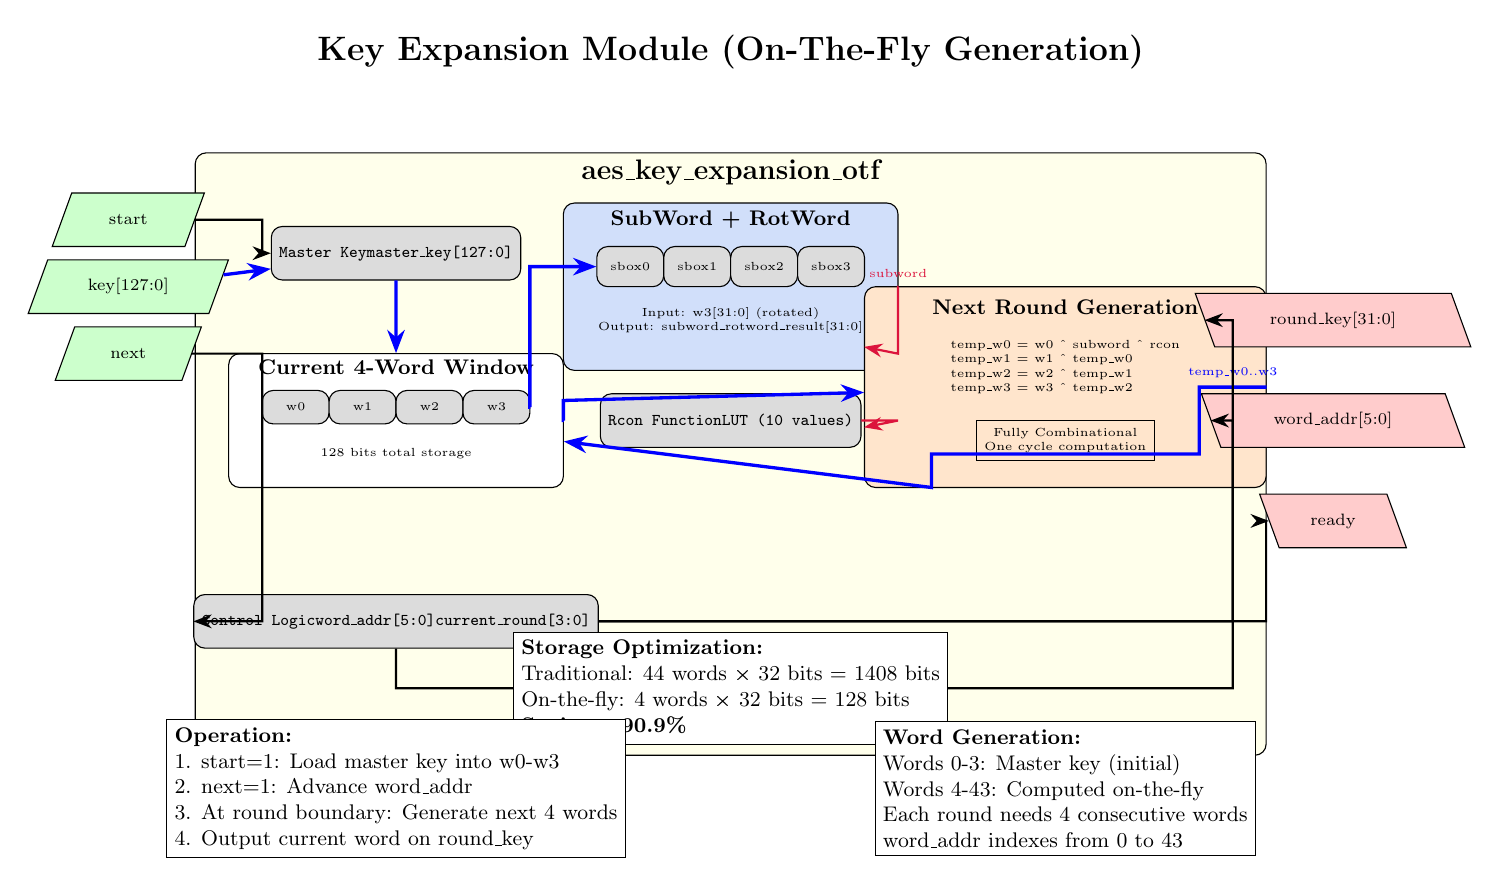
\begin{tikzpicture}[node distance=1.5cm, scale=0.85, every node/.style={transform shape}]

% Title
\node[font=\Large\bfseries] at (0,10) {Key Expansion Module (On-The-Fly Generation)};

% Module boundary
\node[module, minimum width=16cm, minimum height=9cm, fill=keycolor!20] (key_boundary) at (0,4) {};
\node[font=\large\bfseries] at (0,8.2) {aes\_key\_expansion\_otf};

% Inputs
\node[input, font=\scriptsize] (start) at (-9,7.5) {start};
\node[input, font=\scriptsize] (key) at (-9,6.5) {key[127:0]};
\node[input, font=\scriptsize] (next) at (-9,5.5) {next};

% Master key register
\node[submodule, minimum width=3cm] (master_key) at (-5,7) {Master Key\\master\_key[127:0]};

% Current window registers
\node[module, minimum width=5cm, minimum height=2cm, fill=white] (window) at (-5,4.5) {};
\node[font=\small\bfseries] at (-5,5.3) {Current 4-Word Window};
\node[submodule, minimum width=1cm, minimum height=0.5cm, font=\tiny] (w0) at (-6.5,4.7) {w0};
\node[submodule, minimum width=1cm, minimum height=0.5cm, font=\tiny] (w1) at (-5.5,4.7) {w1};
\node[submodule, minimum width=1cm, minimum height=0.5cm, font=\tiny] (w2) at (-4.5,4.7) {w2};
\node[submodule, minimum width=1cm, minimum height=0.5cm, font=\tiny] (w3) at (-3.5,4.7) {w3};
\node[font=\tiny] at (-5,4) {128 bits total storage};

% S-boxes for SubWord/RotWord
\node[module, minimum width=5cm, minimum height=2.5cm] (sbox_array) at (0,6.5) {};
\node[font=\small\bfseries] at (0,7.5) {SubWord + RotWord};
\node[smallmodule, minimum width=1cm, font=\tiny] (sb0) at (-1.5,6.8) {sbox0};
\node[smallmodule, minimum width=1cm, font=\tiny] (sb1) at (-0.5,6.8) {sbox1};
\node[smallmodule, minimum width=1cm, font=\tiny] (sb2) at (0.5,6.8) {sbox2};
\node[smallmodule, minimum width=1cm, font=\tiny] (sb3) at (1.5,6.8) {sbox3};
\node[font=\tiny, align=center] at (0,6) {Input: w3[31:0] (rotated)\\Output: subword\_rotword\_result[31:0]};

% Rcon function
\node[submodule, minimum width=2cm] (rcon) at (0,4.5) {Rcon Function\\LUT (10 values)};

% Combinational logic for next round
\node[module, minimum width=6cm, minimum height=3cm, fill=orange!20] (next_gen) at (5,5) {};
\node[font=\small\bfseries] at (5,6.2) {Next Round Generation};
\node[font=\tiny, align=left] at (5,5.3) {
temp\_w0 = w0 \^{} subword \^{} rcon\\
temp\_w1 = w1 \^{} temp\_w0\\
temp\_w2 = w2 \^{} temp\_w1\\
temp\_w3 = w3 \^{} temp\_w2
};
\node[draw, rectangle, font=\tiny, align=center] at (5,4.2) {Fully Combinational\\One cycle computation};

% Control logic
\node[submodule, minimum width=2.5cm] (control) at (-5,1.5) {Control Logic\\word\_addr[5:0]\\current\_round[3:0]};

% Outputs
\node[output, font=\scriptsize] (round_key_out) at (9,6) {round\_key[31:0]};
\node[output, font=\scriptsize] (word_addr_out) at (9,4.5) {word\_addr[5:0]};
\node[output, font=\scriptsize] (ready_out) at (9,3) {ready};

% Data flow
\draw[bus] (key) -- (master_key);
\draw[arrow] (start) -- (-7,7.5) -- (-7,7) -- (master_key);
\draw[bus] (master_key) -- (window);
\draw[bus] (w3) -- (-3,4.7) -- (-3,6.8) -- (sb0);
\draw[dataarrow] (sbox_array) -- node[above,font=\tiny] {subword} (2.5,6.5) -- (2.5,5.5) -- (next_gen);
\draw[dataarrow] (rcon) -- (2.5,4.5) -- (next_gen);
\draw[bus] (window) -- (-2.5,4.5) -- (-2.5,4.8) -- (next_gen);
\draw[bus] (next_gen) -- node[above,font=\tiny] {temp\_w0..w3} (7,5) -- (7,4) -- (3,4) -- (3,3.5) -- (window);

\draw[arrow] (next) -- (-7,5.5) -- (-7,1.5) -- (control);
\draw[arrow] (control) -- (-5,0.5) -- (7.5,0.5) -- (7.5,6) -- (round_key_out);
\draw[arrow] (control) -- (7.5,1.5) -- (7.5,4.5) -- (word_addr_out);
\draw[arrow] (control) -- (8,1.5) -- (8,3) -- (ready_out);

% Annotations
\node[draw, rectangle, fill=white, align=left, font=\small] at (0,0.5) {
\textbf{Storage Optimization:}\\
Traditional: 44 words × 32 bits = 1408 bits\\
On-the-fly: 4 words × 32 bits = 128 bits\\
\textbf{Savings: 90.9\%}
};

\node[draw, rectangle, fill=white, align=left, font=\small] at (-5,-1) {
\textbf{Operation:}\\
1. start=1: Load master key into w0-w3\\
2. next=1: Advance word\_addr\\
3. At round boundary: Generate next 4 words\\
4. Output current word on round\_key
};

\node[draw, rectangle, fill=white, align=left, font=\small] at (5,-1) {
\textbf{Word Generation:}\\
Words 0-3: Master key (initial)\\
Words 4-43: Computed on-the-fly\\
Each round needs 4 consecutive words\\
word\_addr indexes from 0 to 43
};

\end{tikzpicture}
\caption{On-the-fly key expansion architecture with 90\% storage reduction}
\end{figure}

%==============================================================================
% PAGE 5: Data Path and Round Operations
%==============================================================================
\begin{figure}[p]
\centering
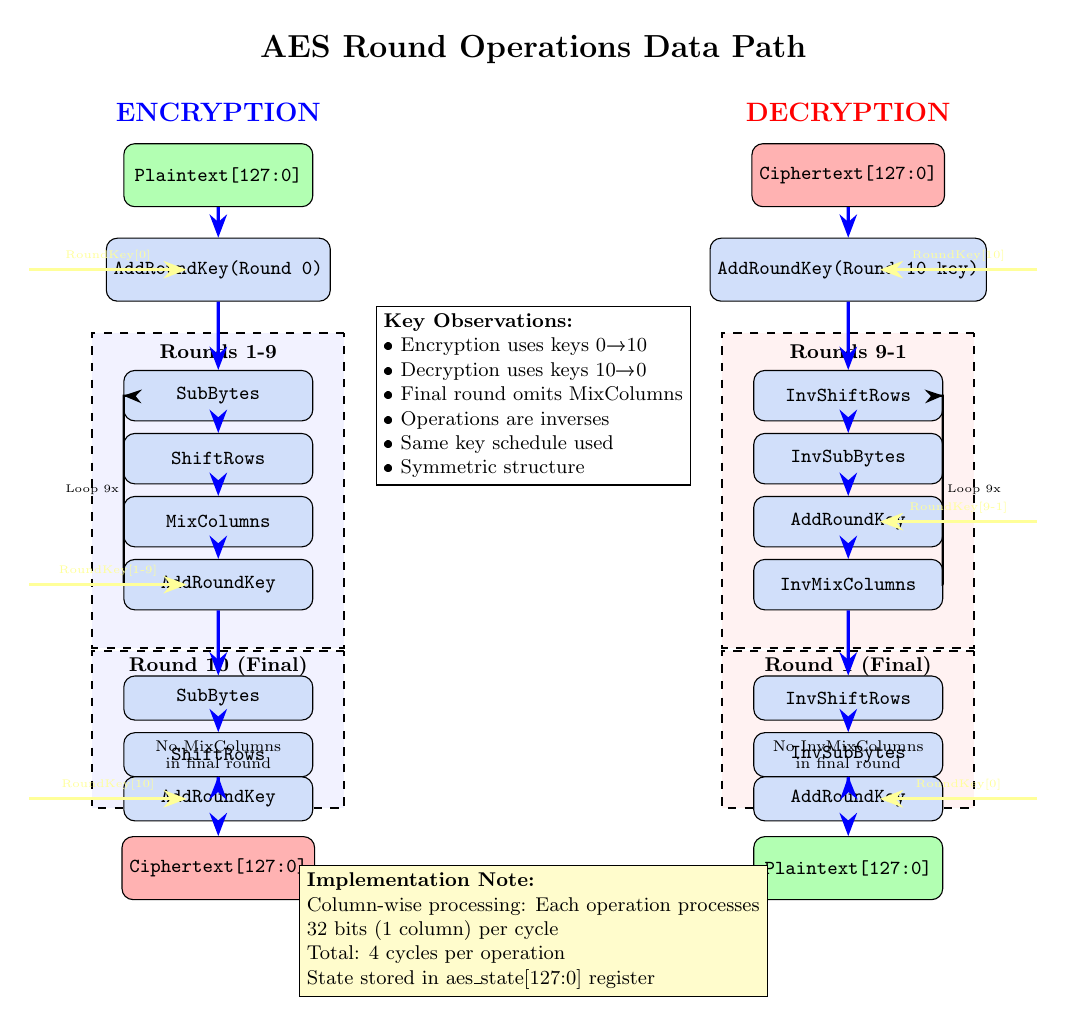
\begin{tikzpicture}[node distance=1.8cm, scale=0.8, every node/.style={transform shape}]

% Title
\node[font=\Large\bfseries] at (0,11) {AES Round Operations Data Path};

% Two columns - Encryption and Decryption
\node[font=\large\bfseries] at (-5,10) {\textcolor{blue}{ENCRYPTION}};
\node[font=\large\bfseries] at (5,10) {\textcolor{red}{DECRYPTION}};

% ENCRYPTION PATH
% Input
\node[module, minimum width=3cm, fill=green!30] (enc_input) at (-5,9) {Plaintext[127:0]};

% Round 0
\node[module, minimum width=3cm] (enc_ark0) at (-5,7.5) {AddRoundKey\\(Round 0)};
\draw[bus] (enc_input) -- (enc_ark0);

% Round 1-9 (loop)
\node[draw, rectangle, minimum width=4cm, minimum height=5cm, dashed, thick, fill=blue!5] (enc_rounds) at (-5,4) {};
\node[font=\small\bfseries] at (-5,6.2) {Rounds 1-9};

\node[module, minimum width=3cm, minimum height=0.8cm] (enc_sub) at (-5,5.5) {SubBytes};
\node[module, minimum width=3cm, minimum height=0.8cm] (enc_shift) at (-5,4.5) {ShiftRows};
\node[module, minimum width=3cm, minimum height=0.8cm] (enc_mix) at (-5,3.5) {MixColumns};
\node[module, minimum width=3cm, minimum height=0.8cm] (enc_ark) at (-5,2.5) {AddRoundKey};

\draw[bus] (enc_ark0) -- (-5,6.5) -- (enc_sub);
\draw[bus] (enc_sub) -- (enc_shift);
\draw[bus] (enc_shift) -- (enc_mix);
\draw[bus] (enc_mix) -- (enc_ark);
\draw[arrow, thick] (enc_ark) -- (-6.5,2.5) -- (-6.5,5.5) -- (enc_sub);
\node[font=\tiny] at (-7,4) {Loop 9x};

% Round 10
\node[draw, rectangle, minimum width=4cm, minimum height=2.5cm, dashed, thick, fill=blue!5] (enc_final) at (-5,0.2) {};
\node[font=\small\bfseries] at (-5,1.2) {Round 10 (Final)};

\node[module, minimum width=3cm, minimum height=0.7cm] (enc_sub10) at (-5,0.7) {SubBytes};
\node[module, minimum width=3cm, minimum height=0.7cm] (enc_shift10) at (-5,-0.2) {ShiftRows};
\node[module, minimum width=3cm, minimum height=0.7cm] (enc_ark10) at (-5,-0.9) {AddRoundKey};

\draw[bus] (enc_ark) -- (-5,1.8) -- (enc_sub10);
\draw[bus] (enc_sub10) -- (enc_shift10);
\draw[bus] (enc_shift10) -- (enc_ark10);

% Output
\node[module, minimum width=3cm, fill=red!30] (enc_output) at (-5,-2) {Ciphertext[127:0]};
\draw[bus] (enc_ark10) -- (enc_output);

% Annotation
\node[font=\scriptsize, align=center] at (-5,-0.2) {No MixColumns\\in final round};

% DECRYPTION PATH
% Input
\node[module, minimum width=3cm, fill=red!30] (dec_input) at (5,9) {Ciphertext[127:0]};

% Round 0
\node[module, minimum width=3cm] (dec_ark0) at (5,7.5) {AddRoundKey\\(Round 10 key)};
\draw[bus] (dec_input) -- (dec_ark0);

% Round 1-9 (loop)
\node[draw, rectangle, minimum width=4cm, minimum height=5cm, dashed, thick, fill=red!5] (dec_rounds) at (5,4) {};
\node[font=\small\bfseries] at (5,6.2) {Rounds 9-1};

\node[module, minimum width=3cm, minimum height=0.8cm] (dec_shift) at (5,5.5) {InvShiftRows};
\node[module, minimum width=3cm, minimum height=0.8cm] (dec_sub) at (5,4.5) {InvSubBytes};
\node[module, minimum width=3cm, minimum height=0.8cm] (dec_ark) at (5,3.5) {AddRoundKey};
\node[module, minimum width=3cm, minimum height=0.8cm] (dec_mix) at (5,2.5) {InvMixColumns};

\draw[bus] (dec_ark0) -- (5,6.5) -- (dec_shift);
\draw[bus] (dec_shift) -- (dec_sub);
\draw[bus] (dec_sub) -- (dec_ark);
\draw[bus] (dec_ark) -- (dec_mix);
\draw[arrow, thick] (dec_mix) -- (6.5,2.5) -- (6.5,5.5) -- (dec_shift);
\node[font=\tiny] at (7,4) {Loop 9x};

% Round 10
\node[draw, rectangle, minimum width=4cm, minimum height=2.5cm, dashed, thick, fill=red!5] (dec_final) at (5,0.2) {};
\node[font=\small\bfseries] at (5,1.2) {Round 1 (Final)};

\node[module, minimum width=3cm, minimum height=0.7cm] (dec_shift10) at (5,0.7) {InvShiftRows};
\node[module, minimum width=3cm, minimum height=0.7cm] (dec_sub10) at (5,-0.2) {InvSubBytes};
\node[module, minimum width=3cm, minimum height=0.7cm] (dec_ark10) at (5,-0.9) {AddRoundKey};

\draw[bus] (dec_mix) -- (5,1.8) -- (dec_shift10);
\draw[bus] (dec_shift10) -- (dec_sub10);
\draw[bus] (dec_sub10) -- (dec_ark10);

% Output
\node[module, minimum width=3cm, fill=green!30] (dec_output) at (5,-2) {Plaintext[127:0]};
\draw[bus] (dec_ark10) -- (dec_output);

% Annotation
\node[font=\scriptsize, align=center] at (5,-0.2) {No InvMixColumns\\in final round};

% Round key annotations
\draw[dataarrow, keycolor, very thick] (-8,7.5) -- node[above,font=\tiny] {RoundKey[0]} (-5.5,7.5);
\draw[dataarrow, keycolor, very thick] (-8,2.5) -- node[above,font=\tiny] {RoundKey[1-9]} (-5.5,2.5);
\draw[dataarrow, keycolor, very thick] (-8,-0.9) -- node[above,font=\tiny] {RoundKey[10]} (-5.5,-0.9);

\draw[dataarrow, keycolor, very thick] (8,7.5) -- node[above,font=\tiny] {RoundKey[10]} (5.5,7.5);
\draw[dataarrow, keycolor, very thick] (8,3.5) -- node[above,font=\tiny] {RoundKey[9-1]} (5.5,3.5);
\draw[dataarrow, keycolor, very thick] (8,-0.9) -- node[above,font=\tiny] {RoundKey[0]} (5.5,-0.9);

% Central notes
\node[draw, rectangle, fill=white, align=left, font=\small] at (0,5.5) {
\textbf{Key Observations:}\\
• Encryption uses keys 0→10\\
• Decryption uses keys 10→0\\
• Final round omits MixColumns\\
• Operations are inverses\\
• Same key schedule used\\
• Symmetric structure
};

\node[draw, rectangle, fill=yellow!20, align=left, font=\small] at (0,-3) {
\textbf{Implementation Note:}\\
Column-wise processing: Each operation processes\\
32 bits (1 column) per cycle\\
Total: 4 cycles per operation\\
State stored in aes\_state[127:0] register
};

\end{tikzpicture}
\caption{Complete data flow for encryption and decryption operations}
\end{figure}

%==============================================================================
% PAGE 6: Column-wise Processing Detail
%==============================================================================
\begin{figure}[p]
\centering
\begin{tikzpicture}[node distance=2cm, scale=0.9, every node/.style={transform shape}]

% Title
\node[font=\Large\bfseries] at (0,11) {Column-wise Processing Architecture};

% State representation
\node[font=\large\bfseries] at (-6,9.5) {128-bit State Matrix};
\node[draw, rectangle, minimum width=5cm, minimum height=5cm, fill=blue!10] (state_matrix) at (-6,6.5) {};

% Draw 4x4 matrix
\foreach \row in {0,1,2,3} {
    \foreach \col in {0,1,2,3} {
        \pgfmathsetmacro{\x}{-7.5 + \col*1.2}
        \pgfmathsetmacro{\y}{8 - \row*1.2}
        \node[draw, rectangle, minimum width=1cm, minimum height=1cm, fill=white] at (\x,\y) {s\textsubscript{\row,\col}};
    }
}

% Highlight columns
\draw[red, very thick, dashed] (-8,8.5) rectangle (-7.3,5);
\node[font=\small, red] at (-7.65,4.5) {Col 0};
\draw[red, very thick, dashed] (-6.8,8.5) rectangle (-6.1,5);
\node[font=\small, red] at (-6.45,4.5) {Col 1};
\draw[red, very thick, dashed] (-5.6,8.5) rectangle (-4.9,5);
\node[font=\small, red] at (-5.25,4.5) {Col 2};
\draw[red, very thick, dashed] (-4.4,8.5) rectangle (-3.7,5);
\node[font=\small, red] at (-4.05,4.5) {Col 3};

\node[font=\small, align=center] at (-6,3.8) {Each column = 32 bits\\(4 bytes)};

% Sequential processing
\node[font=\large\bfseries] at (3,9.5) {Sequential Column Processing};

\node[module, minimum width=2.5cm, minimum height=1.2cm] (col0) at (1,8) {Column 0\\[31:24][23:16]\\[15:8][7:0]};
\node[module, minimum width=2.5cm, minimum height=1.2cm] (col1) at (4,8) {Column 1\\[31:24][23:16]\\[15:8][7:0]};
\node[module, minimum width=2.5cm, minimum height=1.2cm] (col2) at (1,6) {Column 2\\[31:24][23:16]\\[15:8][7:0]};
\node[module, minimum width=2.5cm, minimum height=1.2cm] (col3) at (4,6) {Column 3\\[31:24][23:16]\\[15:8][7:0]};

\draw[arrow, very thick] (col0) -- node[above,font=\small] {cycle 1} (col1);
\draw[arrow, very thick] (col1) -- (5,8) -- (5,6) -- (col3);
\draw[arrow, very thick] (col3) -- node[above,font=\small] {cycle 3} (col2);
\draw[arrow, very thick] (col2) -- (0,6) -- (0,8) -- node[left,font=\small] {cycle 2} (col0);

\node[font=\small] at (2.5,4.8) {4 cycles per operation};

% Processing unit
\node[font=\large\bfseries] at (3,3.5) {32-bit Processing Unit};

\node[module, minimum width=4cm, minimum height=4cm, fill=orange!20] (proc_unit) at (3,0.5) {};

\node[submodule, minimum width=3.5cm] (sub_32) at (3,1.5) {SubBytes\_32bit\\4x S-box lookups};
\node[font=\tiny] at (3,0.8) {OR};
\node[submodule, minimum width=3.5cm] (mix_32) at (3,0.1) {MixColumns\_32bit\\GF(2\textsuperscript{8}) ops};
\node[font=\tiny] at (3,-0.6) {OR};
\node[submodule, minimum width=3.5cm] (ark_32) at (3,-1.3) {AddRoundKey\_32bit\\XOR with round key};

% Input/output
\draw[bus] (2.5,3) -- node[left,font=\small] {32 bits in} (2.5,1.8) -- (sub_32);
\draw[bus] (sub_32) -- (mix_32);
\draw[bus] (mix_32) -- (ark_32);
\draw[bus] (ark_32) -- (3.5,-2) -- node[right,font=\small] {32 bits out} (3.5,-2.5);

% Timing diagram
\node[font=\large\bfseries] at (0,-4) {Timing: 4 cycles per operation};

\node[draw, rectangle, minimum width=1.5cm, minimum height=0.8cm, fill=red!30] at (-4,-5) {Col 0};
\node[draw, rectangle, minimum width=1.5cm, minimum height=0.8cm, fill=red!30] at (-2,-5) {Col 1};
\node[draw, rectangle, minimum width=1.5cm, minimum height=0.8cm, fill=red!30] at (0,-5) {Col 2};
\node[draw, rectangle, minimum width=1.5cm, minimum height=0.8cm, fill=red!30] at (2,-5) {Col 3};

\draw[->] (-5,-5.8) -- (3,-5.8);
\node[font=\small] at (-1,-6.3) {Time (clock cycles) →};

\foreach \i in {0,1,2,3} {
    \pgfmathsetmacro{\x}{-4 + \i*2}
    \node[font=\tiny] at (\x,-5.8) {|\i};
}
\node[font=\tiny] at (3,-5.8) {|4};

% Trade-off table
\node[draw, rectangle, fill=white, align=left, font=\small] at (0,-8) {
\textbf{Design Trade-offs:}\\
\textbf{Parallel (128-bit):} High resources, 1 cycle/op, 4x area\\
\textbf{Column-wise (32-bit):} Low resources, 4 cycles/op, 1x area\\
\textbf{Serial (8-bit):} Minimal resources, 16 cycles/op, 0.25x area\\
\\
\textbf{This design:} Column-wise (balanced approach)
};

% Counter control
\node[draw, rectangle, fill=green!20, align=left, font=\small] at (7,-7) {
\textbf{Control:}\\
col\_cnt[1:0]:\\
\quad 0 → Column 0\\
\quad 1 → Column 1\\
\quad 2 → Column 2\\
\quad 3 → Column 3\\
\\
Increment each cycle\\
Reset when col\_cnt=3
};

\end{tikzpicture}
\caption{Column-wise processing reduces hardware by 75\% with 4x latency increase}
\end{figure}

%==============================================================================
% PAGE 7: Module Interface Summary
%==============================================================================
\begin{figure}[p]
\centering
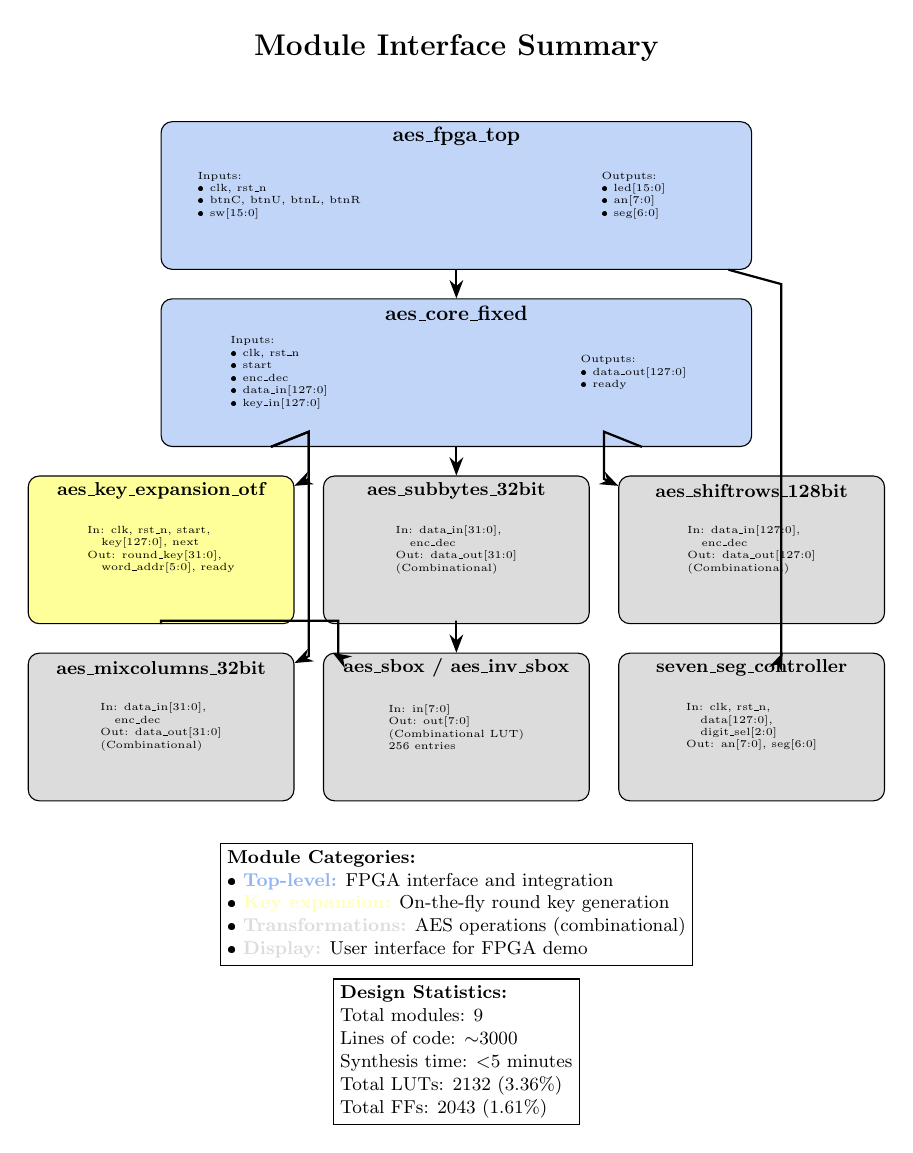
\begin{tikzpicture}[node distance=2cm, scale=0.75, every node/.style={transform shape}]

% Title
\node[font=\Large\bfseries] at (0,13) {Module Interface Summary};

% Top module
\node[module, minimum width=10cm, minimum height=2.5cm, fill=moduleblue!40] (top_mod) at (0,10.5) {};
\node[font=\bfseries] at (0,11.5) {aes\_fpga\_top};
\node[font=\tiny, align=left] at (-3,10.5) {
Inputs:\\
• clk, rst\_n\\
• btnC, btnU, btnL, btnR\\
• sw[15:0]
};
\node[font=\tiny, align=left] at (3,10.5) {
Outputs:\\
• led[15:0]\\
• an[7:0]\\
• seg[6:0]
};

% Core module
\node[module, minimum width=10cm, minimum height=2.5cm, fill=moduleblue!40] (core_mod) at (0,7.5) {};
\node[font=\bfseries] at (0,8.5) {aes\_core\_fixed};
\node[font=\tiny, align=left] at (-3,7.5) {
Inputs:\\
• clk, rst\_n\\
• start\\
• enc\_dec\\
• data\_in[127:0]\\
• key\_in[127:0]
};
\node[font=\tiny, align=left] at (3,7.5) {
Outputs:\\
• data\_out[127:0]\\
• ready
};

% Key expansion
\node[module, minimum width=4.5cm, minimum height=2.5cm, fill=keycolor] (key_mod) at (-5,4.5) {};
\node[font=\small\bfseries] at (-5,5.5) {aes\_key\_expansion\_otf};
\node[font=\tiny, align=left] at (-5,4.5) {
In: clk, rst\_n, start,\\
\quad key[127:0], next\\
Out: round\_key[31:0],\\
\quad word\_addr[5:0], ready
};

% SubBytes
\node[module, minimum width=4.5cm, minimum height=2.5cm, fill=modulegray] (sub_mod) at (0,4.5) {};
\node[font=\small\bfseries] at (0,5.5) {aes\_subbytes\_32bit};
\node[font=\tiny, align=left] at (0,4.5) {
In: data\_in[31:0],\\
\quad enc\_dec\\
Out: data\_out[31:0]\\
(Combinational)
};

% ShiftRows
\node[module, minimum width=4.5cm, minimum height=2.5cm, fill=modulegray] (shift_mod) at (5,4.5) {};
\node[font=\small\bfseries] at (5,5.5) {aes\_shiftrows\_128bit};
\node[font=\tiny, align=left] at (5,4.5) {
In: data\_in[127:0],\\
\quad enc\_dec\\
Out: data\_out[127:0]\\
(Combinational)
};

% MixColumns
\node[module, minimum width=4.5cm, minimum height=2.5cm, fill=modulegray] (mix_mod) at (-5,1.5) {};
\node[font=\small\bfseries] at (-5,2.5) {aes\_mixcolumns\_32bit};
\node[font=\tiny, align=left] at (-5,1.5) {
In: data\_in[31:0],\\
\quad enc\_dec\\
Out: data\_out[31:0]\\
(Combinational)
};

% S-box
\node[module, minimum width=4.5cm, minimum height=2.5cm, fill=modulegray] (sbox_mod) at (0,1.5) {};
\node[font=\small\bfseries] at (0,2.5) {aes\_sbox / aes\_inv\_sbox};
\node[font=\tiny, align=left] at (0,1.5) {
In: in[7:0]\\
Out: out[7:0]\\
(Combinational LUT)\\
256 entries
};

% Seven segment
\node[module, minimum width=4.5cm, minimum height=2.5cm, fill=modulegray] (seg_mod) at (5,1.5) {};
\node[font=\small\bfseries] at (5,2.5) {seven\_seg\_controller};
\node[font=\tiny, align=left] at (5,1.5) {
In: clk, rst\_n,\\
\quad data[127:0],\\
\quad digit\_sel[2:0]\\
Out: an[7:0], seg[6:0]
};

% Connections
\draw[arrow] (top_mod) -- (core_mod);
\draw[arrow] (core_mod) -- (-2.5,6.5) -- (-2.5,5.7) -- (key_mod);
\draw[arrow] (core_mod) -- (sub_mod);
\draw[arrow] (core_mod) -- (2.5,6.5) -- (2.5,5.7) -- (shift_mod);
\draw[arrow] (core_mod) -- (-2.5,6.5) -- (-2.5,2.7) -- (mix_mod);
\draw[arrow] (sub_mod) -- (0,3.3) -- (sbox_mod);
\draw[arrow] (key_mod) -- (-5,3.3) -- (-2,3.3) -- (-2,2.7) -- (sbox_mod);
\draw[arrow] (top_mod) -- (5.5,9) -- (5.5,2.7) -- (seg_mod);

% Summary table
\node[draw, rectangle, fill=white, align=left, font=\small] at (0,-1.5) {
\textbf{Module Categories:}\\
• \textcolor{moduleblue!70}{\textbf{Top-level:}} FPGA interface and integration\\
• \textcolor{keycolor!70}{\textbf{Key expansion:}} On-the-fly round key generation\\
• \textcolor{modulegray}{\textbf{Transformations:}} AES operations (combinational)\\
• \textcolor{modulegray}{\textbf{Display:}} User interface for FPGA demo
};

\node[draw, rectangle, fill=white, align=left, font=\small] at (0,-4) {
\textbf{Design Statistics:}\\
Total modules: 9\\
Lines of code: $\sim$3000\\
Synthesis time: $<$5 minutes\\
Total LUTs: 2132 (3.36\%)\\
Total FFs: 2043 (1.61\%)
};

\end{tikzpicture}
\caption{Complete module hierarchy with interface specifications}
\end{figure}

\end{document}
